%!TEX root = ../main.tex
% ------------------------------------------------------------------------------
\chapter{Theoretical Foundations of Deep Neural Networks}
\label{chapter:dnn-theory}
% ------------------------------------------------------------------------------

\acfp{dnn} have become a powerful class of surrogate models in scientific
computing, particularly for high-dimensional and expensive-to-evaluate
functions. This chapter introduces the mathematical structure and training
procedure of \acp{dnn}, with a focus on activation functions, generalization
theory and gradient-based optimization algorithms. It follows the framework
established in \cite{mishra2021enhancing}.

% ------------------------------------------------------------------------------
\section{Theoretical Foundations of Deep Neural Networks}
\label{sec:dnn-definition}
% ------------------------------------------------------------------------------

The key feature enabling neural networks to approximate nonlinear functions is
the application of scalar activation functions. We begin by introducing these
components before defining the class of functions represented by \aclp{dnn}.

\begin{definition}[Activation Function] \ \\
An \emph{activation function} is a measurable function $\sigma : \mathbb{R} \to
\mathbb{R}$, typically nonlinear, that is applied componentwise to the output of
each layer in a neural network. For a vector $z = (z_1, \dots, z_k)^\top \in
\mathbb{R}^k$, the activation is defined as
\begin{equation*}
    \sigma(z) := (\sigma(z_1), \dots, \sigma(z_k))^\top.
\end{equation*}
\end{definition}

\begin{example}[Common Activation Functions] \ \\
Two widely used activation functions are illustrated in
Figure~\ref{fig:activation_functions}. These are also the activation functions
we employ in the experimental evaluations presented in Chapter~\ref{chapter7}.

\begin{itemize}
    \item \textbf{ReLU (Rectified Linear Unit)}:
    \begin{equation*}
        \sigma(z) = \max\{0, z\}
    \end{equation*}
    ReLU is piecewise linear and unbounded. It is computationally efficient and
    commonly used in deep architectures.
    
    \item \textbf{Sigmoid}:
    \begin{equation*}
        \sigma(z) = \frac{1}{1 + e^{-z}}
    \end{equation*}
    The sigmoid function maps real numbers to $(0,1)$ and is differentiable
    everywhere. It is often used in theoretical analysis and binary
    classification tasks.
\end{itemize}
\end{example}

\begin{figure}[H]
  \centering
  \includegraphics[width=0.95\textwidth]{Figures/activations_functions.png}
  \caption{Comparison of ReLU and Sigmoid activation functions.}
  \label{fig:activation_functions}
\end{figure}

With an activation function in place, we now define the class of functions that
a fully connected feedforward neural network can represent.

\begin{definition}[Class of Deep Neural Network Functions] \ \\
Let $L \in \mathbb{N}$ and $\mathbf{d} = (d_0, d_1, \dots, d_L)$ be a sequence
of positive integers, where $d_0 = s$ is the input dimension and $d_L = 1$ the
output dimension. A \acf{dnn} of \emph{depth} $L$ and \emph{layer widths} $d_1,
\dots, d_{L-1}$ is a function $f_\theta: \mathbb{R}^s \to \mathbb{R}$ of the
form
\begin{equation*}
    f_\theta(y) = A_L \circ \sigma \circ A_{L-1} \circ \cdots \circ \sigma \circ A_1(y),
\end{equation*}
where each \emph{layer map} $A_l: \mathbb{R}^{d_{l-1}} \to \mathbb{R}^{d_l}$ is
an affine transformation
\begin{equation*}
    A_l(z) = W_l z + b_l,
\end{equation*}
with weights $W_l \in \mathbb{R}^{d_l \times d_{l-1}}$ and biases $b_l \in
\mathbb{R}^{d_l}$. The activation function $\sigma: \mathbb{R} \to \mathbb{R}$
is applied component-wise.

The collection of all trainable parameters is denoted by
\begin{equation*}
\theta = \{ (W_l, b_l) \}_{l=1}^L,
\end{equation*}
and fully determines the function $f_\theta$. The set of all such realizable
functions for a given architecture and activation $\sigma$ is denoted by
$\mathcal{F}_{L, \mathbf{d}, \sigma}$.

\vspace{0.5em}
\noindent The architectural parameters are interpreted as follows:
\begin{itemize}
    \item The \emph{depth} $L$ is the number of affine layers.
    \item The \emph{width} $d_l$ specifies the number of neurons in layer $l$.
    \item The \emph{layer structure} is encoded in the tuple $\mathbf{d}$.
\end{itemize}
\end{definition}


In the course of this work, we assume that all hidden layers have the same
number of neurons, i.e., the network has constant width $m$ for all layers $l =
1, \dots, L-1$. In Figure~\ref{fig:dnn-architecture}, a fully connected \ac{dnn}
with constant width is illustrated.

\begin{figure}[H]
\centering
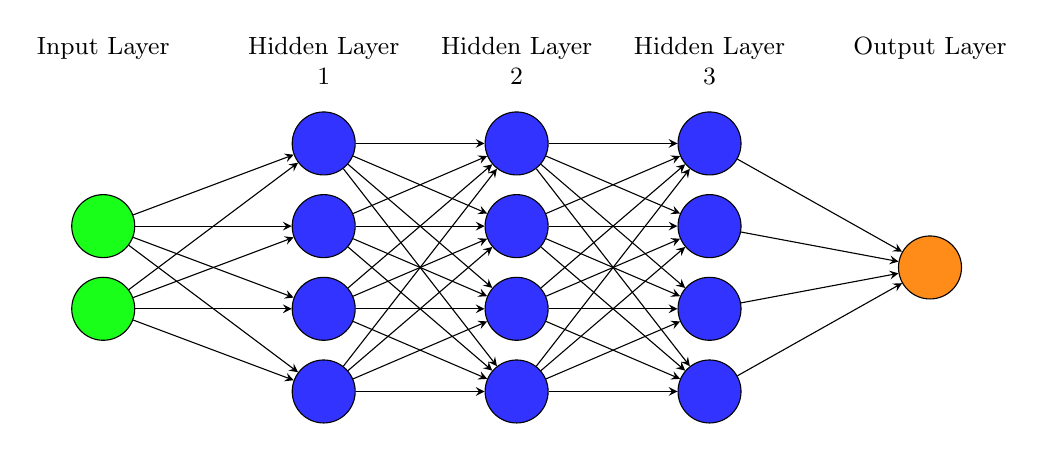
\begin{tikzpicture}[scale=.7, align=center, neuron/.style={circle, draw=black,
  minimum size=.8cm}, layer/.style={draw=none, minimum height=1.5cm}, every
  node/.style={font=\small} ]


% Layer labels
\node at (-7.5,.5) {Input Layer\\ }; \node at (-3.5,.5) {Hidden Layer\\ 1};
\node at (0,.5) {Hidden Layer\\ 2}; \node at (3.5,.5) {Hidden Layer\\ 3}; \node
at (7.5,.5) {Output Layer\\ };

% Input layer
\foreach \i in {1,2} { \node[neuron, fill=green, fill opacity=0.9] (I\i) at
  (-7.5,-\i*1.5-1) {}; }

% Hidden layer 1
\foreach \i in {1,2,3,4} { \node[neuron, fill=blue, fill opacity=0.8] (H1\i) at
  (-3.5,-\i*1.5+0.5) {}; }

% Hidden layer 2
\foreach \i in {1,2,3,4} { \node[neuron, fill=blue, fill opacity=0.8] (H2\i) at
  (0,-\i*1.5+0.5) {}; }

% Hidden layer 3
\foreach \i in {1,2,3,4} { \node[neuron, fill=blue, fill opacity=0.8] (H3\i) at
  (3.5,-\i*1.5+0.5) {}; }

% Output layer

\node[neuron, fill=orange, fill opacity=0.9] (O1) at (7.5,-3.25) {};


% Connections input -> hidden 1
\foreach \i in {1,2} \foreach \j in {1,2,3,4} \draw[-stealth] (I\i) -- (H1\j);

% hidden 1 -> hidden 2
\foreach \i in {1,2,3,4} \foreach \j in {1,2,3,4} \draw[-stealth] (H1\i) --
  (H2\j);

% hidden 2 -> hidden 3
\foreach \i in {1,2,3,4} \foreach \j in {1,2,3,4} \draw[-stealth] (H2\i) --
  (H3\j);

% hidden 3 -> output
\foreach \i in {1,2,3,4} \draw[-stealth] (H3\i) -- (O1);

\end{tikzpicture}
\caption{Schematic of a fully connected \aclp{dnn} with constant width $m=4$ and
depth $L=3$ layers.}
\label{fig:dnn-architecture}
\end{figure}


\begin{remark}
    For the layer structure $d=(d_0,...,d_L)$, the total number of trainable
    parameters (weights and biases) of $theta$ in the network is given by
    \begin{equation*}
        N_\theta = \sum_{l=1}^{L} (d_{l-1} \cdot d_l + d_l) = (L-2) \cdot m^2 + (L+s) \cdot m + 1.
    \end{equation*}
    
\end{remark}

% ------------------------------------------------------------------------------
\section{Training and Generalization Error}
\label{sec:dnn-error}
% ------------------------------------------------------------------------------

Supervised training of a \ac{dnn} requires minimizing the discrepancy between
the network output $f_\theta(y)$ and a ground truth map $L(y)$ on a given
training set $\{y_i\}_{i=1}^N$.

\begin{definition}[Training Error] \ \\
The empirical risk or training error is defined by
 \begin{equation*}
\mathcal{E}_\mathrm{T}(\theta) = \frac{1}{N} \sum_{i=1}^N |L(y_i) - f_\theta(y_i)|.
 \end{equation*}
\end{definition}

\begin{definition}[Generalization Error] \ \\
The generalization error (or population risk) is the expected error under the
data distribution $\mu$:
 \begin{equation*}
\mathcal{E}_\mathrm{G}(\theta) = \int_{\mathcal{Y}} |L(y) - f_\theta(y)| \, \mathrm{d}\mu(y).
 \end{equation*}
\end{definition}


% ------------------------------------------------------------------------------
\section{Optimization and Training Procedures}
\label{sec:dnn-training}
% ------------------------------------------------------------------------------

Training a \ac{dnn} corresponds to solving the following regularized
minimization problem:

\begin{equation}
    \theta^* = \arg\min_{\theta \in \Theta} \left[ \mathcal{E}_\mathrm{T}(\theta) + \lambda \cdot R(\theta) \right],
    \label{eq:regularized-objective}
\end{equation}

where $R(\theta)$ is a regularization term (e.g., $\ell^2$ weight penalty) and
$\lambda > 0$ controls its strength.

% hier kommt schema
\begin{figure}[htbp]
\centering
\begin{tikzpicture}[
    node distance=1.8cm and 3.2cm,
    every node/.style={font=\small},
    process/.style={rectangle, draw, thick, align=center, minimum width=4.6cm, minimum height=1.1cm, fill=gray!10},
    io/.style={rectangle, draw, thick, align=center, minimum width=4.6cm, minimum height=1.1cm, fill=blue!10},
    decision/.style={diamond, draw, thick, aspect=2, align=center, inner sep=0pt, minimum width=3.5cm, fill=orange!15},
    result/.style={rectangle, draw, thick, align=center, minimum width=4.6cm, minimum height=1.1cm, fill=green!15},
    arrow/.style={->, thick},
]

% Nodes
\node[io] (input) {Input: Map $L$ and\\ low-discrepancy sequence $(y_n)_{n=1}^N$};
\node[process, below=of input] (step1) {Step 1:\\ Evaluate $L(y_n)$ for all $y_n \in S \subset Y$};
\node[process, below=of step1] (step2) {Step 2:\\ Initialize NN $L_\theta$,\\ compute loss and gradients};
\node[process, below=of step2] (step3) {Step 3:\\ Run SGD to minimize loss};
\node[result, below=of step3] (output) {Output: Trained NN $L^* = L_{\theta^*}$ approximates $L$};

% Arrows
\draw[arrow] (input) -- (step1);
\draw[arrow] (step1) -- (step2);
\draw[arrow] (step2) -- (step3);
\draw[arrow] (step3) -- (output);

% Optional annotation on side
\node[align=left, font=\footnotesize, right=3.8cm of step1, text width=4.6cm] (note1) {
    \textbf{Note:}\\
    $S = \{y_n\}$ is chosen\\
    as a low-discrepancy sequence.
};

\node[align=left, font=\footnotesize, right=3.8cm of step2, text width=4.6cm] (note2) {
    \textbf{SGD Initialization:}\\
    Use $\nabla_\theta \mathcal{L}(L_\theta(y_n), L(y_n))$.
};

\end{tikzpicture}
\caption{Workflow of Algorithm 2.2: Deep learning of parameters-to-observable map using low-discrepancy sampling and SGD-based training.}
\label{fig:algo22_dnn_training}
\end{figure}


\subsection{Stochastic Gradient Descent (SGD)}

In practice, \eqref{eq:regularized-objective} is minimized via stochastic
gradient descent:

 \begin{equation*}
\theta_{t+1} = \theta_t - \eta \cdot \nabla_\theta \mathcal{E}_\mathrm{T}^{(B)}(\theta_t),
 \end{equation*}

where $\eta$ is the learning rate and $\mathcal{E}_\mathrm{T}^{(B)}$ is the
mini-batch loss.

\subsection{Adam Optimizer}

The Adam algorithm improves on SGD by incorporating adaptive learning rates and
momentum:

\begin{algorithm}[H]
\caption{Adam Optimizer (simplified)}
\begin{algorithmic}[1]
\State Initialize $\theta_0$, $m_0 = 0$, $v_0 = 0$ \For{$t = 1$ to $T$} \State
$g_t \gets \nabla_\theta \mathcal{E}_T(\theta_{t-1})$ \State $m_t \gets \beta_1
m_{t-1} + (1 - \beta_1) g_t$ \State $v_t \gets \beta_2 v_{t-1} + (1 - \beta_2)
g_t^2$ \State $\hat{m}_t \gets m_t / (1 - \beta_1^t)$ \State $\hat{v}_t \gets
v_t / (1 - \beta_2^t)$ \State $\theta_t \gets \theta_{t-1} - \eta \cdot
\hat{m}_t / (\sqrt{\hat{v}_t} + \epsilon)$ \EndFor
\end{algorithmic}
\end{algorithm}

\begin{remark}
The Adam optimizer is particularly effective in early training and in
high-dimensional, noisy settings. Its convergence properties, however, require
careful tuning of $\beta_1$, $\beta_2$ and $\epsilon$.
\end{remark}




































\chapter{Theoretical Foundations of QMC-Based Learning}
\label{chapter5}

\begin{itemize}
    \item Adapting QMC theory to supervised learning
    \item Hardy-Krause variation of the loss function
    \item Generalization error bounds using low-discrepancy samplin\item 
    \item Comparison to MC-based bounds and practical implication\item 
    \item Validity conditions and smoothness assumptions
\end{itemize}

\begin{align*}
    V_{\mathrm{HK}}(f) = V_{\mathrm{HK}}(f; a, b) &= \sum_{u\subset \{1,\dots,s\}} V_{[a^{-u}, b^{-u}]} f(x^{-u}:b^u) \\
    &= \sum_{u\subset \{1,\dots,s\}} \sup_{\mathcal{Y} \in \mathbb{Y}} V_\mathcal{Y} \big( f(x^{-u} : b^u) \big) \\
    &= \sum_{u\subset \{1,\dots,s\}} \sup_{\mathcal{Y} \in \mathbb{Y}} \sum_{y\in\mathcal{Y}} \big| \Delta\big( f(x^{-u} : b^u); y, y_+ \big) \big| \\
    &= \sum_{u\subset \{1,\dots,s\}} \sup_{\mathcal{Y} \in \mathbb{Y}} \sum_{y\in\mathcal{Y}} \big| \sum_{v\subseteq \{1,\dots,s\}} (-1)^{|v|} f((y^v:y_+^{-v})^{-u}:b^{u}) \big| \\
\end{align*}

For the definitions of Variation we follow \cite{owen2005multidimensional} and
start by introducing the mixed power notation:

\begin{definition}[Mixed Component Selection] \ \\
    \label{def:component_merge}
    Let $\boldsymbol{a}, \boldsymbol{b} \in \mathbb{R}^s$ and let $u \subseteq
    \{1, \dots, s\}$ be an index set. We define
    \begin{equation*}
        \boldsymbol{c} := \boldsymbol{a}^u : \boldsymbol{b}^{-u}
        \quad \text{with} \quad
        c_j := 
        \begin{cases}
            a_j, & \text{if } j \in u, \\
            b_j, & \text{if } j \notin u.
        \end{cases}
    \end{equation*}
\end{definition}

Hereby the term $-u$ denotes the complement of $u$ in $\{1, \dots, s\}$. Further
the alternating sum is defined.

\begin{definition}[Alternating sum] \ \\
    The \emph{alternating sum} on $s$ dimensions with respect to a function on
    the hyperrectangle $[a,b]$ is defined as
    \begin{equation*}
        \Delta(f; a, b) = \sum_{v \subseteq \{1,\dots,s\}} (-1)^{|v|} f(a^v:b^{-v}).
    \end{equation*}
\end{definition}

An essential concept in this context is the notion of a \emph{ladder} which we
define on a certain hypercube $[a,b]$.

\begin{definition}[Ladder] \ \\
    A \emph{ladder} on the hypercube $[a,b]$ is a set of points $\mathcal{Y} =
    \{y_1, \dots, y_k\} \subset [a,b]$ such that for each $i < j$, the point
    $y_i$ is less than or equal to $y_j$ in every coordinate. Formally, this
    means that for all $i < j$ and for all $l \in \{1, \dots, s\}$, we have
    $y_i^l \leq y_j^l$.
\end{definition}

The space of all such ladders on the hypercube is denoted by $\mathbb{Y}$. Next,
the \emph{variation with respect to a ladder} is defined.

\begin{definition}[Variation with respect to a ladder] \ \\
    The \emph{variation} of a function $f$ on the hyperrectangle $[a,b]$
    \emph{with respect to a ladder}
    $\mathcal{Y} = \prod\limits_{j=1}^s \mathcal{Y}^j$ is defined as
    \begin{equation*}
        V_\mathcal{Y}(f) = \sum_{y \in \mathcal{Y}} \big| \Delta(f; y, y_+) \big|,
    \end{equation*}
    where $y_+$ is the point obtained by incrementing each coordinate of $y$
    with $y^j_+$ to be the successor of $y_j$ in $\mathcal{Y}^j$.
\end{definition}

Accordingly the Variation by Vitali is defined as the supremum of the variation
over all ladders $\mathcal{Y} \in \mathbb{Y}$.

\begin{definition}[Vitali Variation] \ \\
    The \emph{Vitali variation} of a function $f$ on the hyperrectangle $[a,b]$
    is defined as
    \begin{equation*}
        V(f) = V(f; a, b) = \sup_{\mathcal{Y} \in \mathbb{Y}} V_\mathcal{Y}(f).
    \end{equation*}
    Here $\mathbb{Y}$ denotes the set of all ladders on the hyperrectangle
    $[a,b]$.
\end{definition}

The Hardy--Krause variation is a specific case of the Vitali variation, where
the supremum is taken over all ladders in the unit hypercube $[0,1]^s$.

\begin{definition}[Hardy--Krause Variation] \ \\
    The \emph{Hardy--Krause variation} of a function $f$ on the hyperrectangle
    $[a,b]$ is defined as
    \begin{equation*}
        V_{\mathrm{HK}}(f) = V_{\mathrm{HK}}(f; 0, 1) = \sup_{\mathcal{Y} \in 
        \mathbb{Y}} V_\mathcal{Y}(f).
    \end{equation*}
\end{definition}




% % Chapter Template

% \chapter{Neural Network Training for Stochastic Functions} % Main chapter
% title

% \label{Chapter4} % Change X to a consecutive number; for referencing this
% chapter elsewhere, use \ref{ChapterX}

% %----------------------------------------------------------------------------------------
% % SECTION 1
% %----------------------------------------------------------------------------------------

% \section{Modeling Randomness in Physical Simulations}

% Lorem ipsum dolor sit amet, consectetur adipiscing elit. Aliquam ultricies
% lacinia euismod. Nam tempus risus in dolor rhoncus in interdum enim tincidunt.
% Donec vel nunc neque. In condimentum ullamcorper quam non consequat. Fusce
% sagittis tempor feugiat. Fusce magna erat, molestie eu convallis ut, tempus
% sed arcu. Quisque molestie, ante a tincidunt ullamcorper, sapien enim
% dignissim lacus, in semper nibh erat lobortis purus. Integer dapibus ligula ac
% risus convallis pellentesque.

% %----------------------------------------------------------------------------------------
% % SECTION 2
% %----------------------------------------------------------------------------------------

% \section{Sampling Stochastic Variables with QMC and MC}

% Sed ullamcorper quam eu nisl interdum at interdum enim egestas. Aliquam
% placerat justo sed lectus lobortis ut porta nisl porttitor. Vestibulum mi
% dolor, lacinia molestie gravida at, tempus vitae ligula. Donec eget quam
% sapien, in viverra eros. Donec pellentesque justo a massa fringilla non
% vestibulum metus vestibulum. Vestibulum in orci quis felis tempor lacinia.
% Vivamus ornare ultrices facilisis. Ut hendrerit volutpat vulputate. Morbi
% condimentum venenatis augue, id porta ipsum vulputate in. Curabitur luctus
% tempus justo. Vestibulum risus lectus, adipiscing nec condimentum quis,
% condimentum nec nisl. Aliquam dictum sagittis velit sed iaculis. Morbi
% tristique augue sit amet nulla pulvinar id facilisis ligula mollis. Nam elit
% libero, tincidunt ut aliquam at, molestie in quam. Aenean rhoncus vehicula
% hendrerit.

% %----------------------------------------------------------------------------------------
% % SECTION 3
% %----------------------------------------------------------------------------------------

% \section{Data Generation: Simulating Photon Scatter}

% Sed ullamcorper quam eu nisl interdum at interdum enim egestas. Aliquam
% placerat justo sed lectus lobortis ut porta nisl porttitor. Vestibulum mi
% dolor, lacinia molestie gravida at, tempus vitae ligula. Donec eget quam
% sapien, in viverra eros. Donec pellentesque justo a massa fringilla non
% vestibulum metus vestibulum. Vestibulum in orci quis felis tempor lacinia.
% Vivamus ornare ultrices facilisis. Ut hendrerit volutpat vulputate. Morbi
% condimentum venenatis augue, id porta ipsum vulputate in. Curabitur luctus
% tempus justo. Vestibulum risus lectus, adipiscing nec condimentum quis,
% condimentum nec nisl. Aliquam dictum sagittis velit sed iaculis. Morbi
% tristique augue sit amet nulla pulvinar id facilisis ligula mollis. Nam elit
% libero, tincidunt ut aliquam at, molestie in quam. Aenean rhoncus vehicula
% hendrerit.

% %----------------------------------------------------------------------------------------
% % SECTION 4
% %----------------------------------------------------------------------------------------

% \section{Learning Setup and Experimental Design}

% Sed ullamcorper quam eu nisl interdum at interdum enim egestas. Aliquam
% placerat justo sed lectus lobortis ut porta nisl porttitor. Vestibulum mi
% dolor, lacinia molestie gravida at, tempus vitae ligula. Donec eget quam
% sapien, in viverra eros. Donec pellentesque justo a massa fringilla non
% vestibulum metus vestibulum. Vestibulum in orci quis felis tempor lacinia.
% Vivamus ornare ultrices facilisis. Ut hendrerit volutpat vulputate. Morbi
% condimentum venenatis augue, id porta ipsum vulputate in. Curabitur luctus
% tempus justo. Vestibulum risus lectus, adipiscing nec condimentum quis,
% condimentum nec nisl. Aliquam dictum sagittis velit sed iaculis. Morbi
% tristique augue sit amet nulla pulvinar id facilisis ligula mollis. Nam elit
% libero, tincidunt ut aliquam at, molestie in quam. Aenean rhoncus vehicula
% hendrerit.

% %----------------------------------------------------------------------------------------
% % SECTION 5
% %----------------------------------------------------------------------------------------

% \section{Convergence and Performance Comparison}

% Sed ullamcorper quam eu nisl interdum at interdum enim egestas. Aliquam
% placerat justo sed lectus lobortis ut porta nisl porttitor. Vestibulum mi
% dolor, lacinia molestie gravida at, tempus vitae ligula. Donec eget quam
% sapien, in viverra eros. Donec pellentesque justo a massa fringilla non
% vestibulum metus vestibulum. Vestibulum in orci quis felis tempor lacinia.
% Vivamus ornare ultrices facilisis. Ut hendrerit volutpat vulputate. Morbi
% condimentum venenatis augue, id porta ipsum vulputate in. Curabitur luctus
% tempus justo. Vestibulum risus lectus, adipiscing nec condimentum quis,
% condimentum nec nisl. Aliquam dictum sagittis velit sed iaculis. Morbi
% tristique augue sit amet nulla pulvinar id facilisis ligula mollis. Nam elit
% libero, tincidunt ut aliquam at, molestie in quam. Aenean rhoncus vehicula
% hendrerit.